\chapter{Specifikacija programske potpore}

\section{Funkcionalni zahtjevi}

    \noindent \textbf{Dionici:}

\begin{packed_enum}
	
	\item Vlasnik
	\item Adminikstrator				
	\item Korisnici
	\item Razvojni tim

	
\end{packed_enum}

\noindent \textbf{Aktori i njihovi funkcionalni zahtjevi:}


\begin{packed_enum}

	\item  \underbar{Vlasnik (inicijator) može:}
	
	\begin{packed_enum}
		
		\item mijenjati podatke u sustavu
		\item definirati administratore sustava
		\item pregledati podatke o posjećenosti stranice
		\item vidjeti odvojeni prikaz broja pregleda stranice
		\item vidjeti podatke o reprodukciji zvučnih zapisa
		
	\end{packed_enum}

	\item  \underbar{Administrator (inicijator) može:}
	
	\begin{packed_enum}
		
		\item uređivati podatke o izlošcima i objektima muzeja
		\item postaviti zvučne zapise
		\item pregledati podatke o posjećenosti stranice
		\item vidjeti odvojeni prikaz broja pregleda stranice
		\item vidjeti podatke o reprodukciji zvučnih zapisa
		
	\end{packed_enum}

	\item  \underbar{Registrirani korisnik (inicijator) može:}
	
	\begin{packed_enum}
		
		\item pregledati podatke o objektima i izlošcima
		\item pokrenuti zvučne zapise
		\item primati promo materijale turističke zajednice
		
	\end{packed_enum}
\newpage
		\item  \underbar{Neregistrirani korisnik (inicijator) može:}
	
	\begin{packed_enum}
		
		\item pregledati podatke o objektima i izlošcima
		\item pokrenuti zvučne zapise
		
	\end{packed_enum}
	
	\item  \underbar{Baza podataka (sudionik) sadrži:}
	
	\begin{packed_enum}
		
		\item podatke o korisnicima sustava
		\item podatke o objektima i izlošcima
		\item zvučne zapise
		\item podatke o izvješćima
		
	\end{packed_enum}
\end{packed_enum}


\eject 



\subsection{Obrasci uporabe}

\subsubsection{Opis obrazaca uporabe}


	\noindent \underbar{\textbf{UC$<$1$>$ -$<$Pregled svih muzejskih objekata$>$}}
	\begin{packed_item}
		
		\item \textbf{Glavni sudionik: }$<$Neregistrirani korisnik$>$
		\item  \textbf{Cilj:} $<$Pregledati muzejske objekte$>$
		\item  \textbf{Sudionici:} $<$Baza podataka$>$
		\item  \textbf{Preduvjet:} $<$-$>$
		\item  \textbf{Opis osnovnog tijeka:}
		
		\item[] \begin{packed_enum}
			
			\item $<$Učitavanjem aplikacije prikazuju se muzejski objekti i njihova imena.$>$
			\item $<$Prikazuje se slika i ime muzejskog objekta$>$
		\end{packed_enum}
		
	\end{packed_item}
	
	\noindent \underbar{\textbf{UC$<$2$>$ -$<$Pregled muzejskog objekta$>$}}
	\begin{packed_item}
		
		\item \textbf{Glavni sudionik: }$<$Neregistrirani korisnik$>$
		\item  \textbf{Cilj:} $<$Pregledati muzejski objekt$>$
		\item  \textbf{Sudionici:} $<$Baza podataka$>$
		\item  \textbf{Preduvjet:} $<$-$>$
		\item  \textbf{Opis osnovnog tijeka:}
		
		\item[] \begin{packed_enum}
			
			\item $<$Korisnik odabire muzejski objekt$>$
			\item $<$Otvara se stranica odabranog muzejskog objekta$>$
			\item $<$Prikazuje se ime, slika, opis i zvučni zapis odabranog muzejskog objekta$>$
		\end{packed_enum}
		
	\end{packed_item}
	
	\noindent \underbar{\textbf{UC$<$3$>$ -$<$Registracija$>$}}
	\begin{packed_item}
		
		\item \textbf{Glavni sudionik: }$<$Neregistrirani korisnik$>$
		\item  \textbf{Cilj:} $<$Stvoriti korisnički račun za pristup sustavu$>$
		\item  \textbf{Sudionici:} $<$Baza podataka$>$
		\item  \textbf{Preduvjet:} $<$-$>$
		\item  \textbf{Opis osnovnog tijeka:}
		
		\item[] \begin{packed_enum}
			
			\item $<$Korisnik odabire opciju za registraciju$>$
			\item $<$Korisnik unosi potrebne korisničke podatke$>$
			\item $<$Korisnik prima pozdravnu poruku i traži se potvrda klikom na link$>$
			\item $<$Korisnik prima prima pristupne podatke na adresu elektroničke pošte$>$
			\item $<$Promjene se upisuju u bazu podataka$>$
		\end{packed_enum}
		
		\item  \textbf{Opis mogućih odstupanja:}
		
		\item[] \begin{packed_item}
			
			\item[2.a] $<$Odabir već zauzetog korisničkog imena i/ili e-maila, unos korisničkog podatka u nedozvoljenom formatu ili pružanje neispravnoga e-maila$>$
			\item[] \begin{packed_enum}
				
				\item $<$Sustav obavještava korisnika o neuspjelom upisu i vraća ga na stranicu za registraciju$>$
				\item $<$Korisnik mijenja potrebne podatke te završava unos ili odustaje od registracije$>$
				
			\end{packed_enum}
			
		\end{packed_item}
	\end{packed_item}
	
	\noindent \underbar{\textbf{UC$<$4$>$ -$<$Prijava korisnika$>$}}
	\begin{packed_item}
		
		\item \textbf{Glavni sudionik: }$<$Registrirani korisnik$>$
		\item  \textbf{Cilj:} $<$Prijaviti se u sustav$>$
		\item  \textbf{Sudionici:} $<$Baza podataka$>$
		\item  \textbf{Preduvjet:}$<$Uspješna registracija korisnika u sustav, mogućnost spajanja na internet$>$
		\item  \textbf{Opis osnovnog tijeka:}
		
		\item[] \begin{packed_enum}
			
			\item $<$Odabir opcije prijavi se$>$
			\item $<$Unos korisničkog imena i lozinke$>$
			\item $<$Potvrda o ispravnosti unesenih podataka$>$
			\item $<$Pristup korisničkim funkcijama$>$
		\end{packed_enum}
		
		\item  \textbf{Opis mogućih odstupanja:}
		
		\item[] \begin{packed_item}
			
			\item[2.a] $<$Neispravno korisničko ime ili lozinka$>$
			\item[] \begin{packed_enum}
				
				\item $<$Sustav obavještava korisnika o neuspjeloj prijavi i vraća ga na stranicu za prijavu$>$
				
			\end{packed_enum}
			
		\end{packed_item}
	\end{packed_item}

	\noindent \underbar{\textbf{UC$<$5$>$ -$<$Skeniranje QR koda$>$}}
	\begin{packed_item}
		
		\item \textbf{Glavni sudionik: }$<$Neregistrirani korisnik$>$
		\item  \textbf{Cilj:} $<$Pokrenuti zvučni zapis$>$
		\item  \textbf{Sudionici:} $<$Baza podataka$>$
		\item  \textbf{Preduvjet:} $<$Mogućnost korištenja kamere na mobilnom uređaju$>$
		\item  \textbf{Opis osnovnog tijeka:}
		
		\item[] \begin{packed_enum}
			
			\item $<$Odabir izložbenog objekta s početne stranice$>$
			\item $<$Postavljanje mobilnog uređaja tako da se QR kod prikaže u tražilu aplikacije Kamera$>$
			\item $<$Dotaknuti obavijest kako bi se otvorila veza povezana s QR kodom$>$
		\end{packed_enum}	
	\end{packed_item}

	\noindent \underbar{\textbf{UC$<$6$>$ -$<$Dohvat promotivnih materijala$>$}}
	\begin{packed_item}
		
		\item \textbf{Glavni sudionik: }$<$Registrirani korisnik$>$
		\item  \textbf{Cilj:} $<$Dohvatiti promotivne materijale$>$
		\item  \textbf{Sudionici:} $<$Baza podataka$>$
		\item  \textbf{Preduvjet:} $<$Korisnik je prijavljen$>$
		\item  \textbf{Opis osnovnog tijeka:}
		
		\item[] \begin{packed_enum}
			
			\item $<$Korisnik odabire opciju za dohvat promotivnih materijala$>$
			\item $<$Aplikacija prikazuje promotivne materijale$>$

		\end{packed_enum}
	\end{packed_item}

	\noindent \underbar{\textbf{UC$<$7$>$ -$<$Pregled osobnih podataka$>$}}
	\begin{packed_item}
		
		\item \textbf{Glavni sudionik: }$<$Registrirani korisnik$>$
		\item  \textbf{Cilj:} $<$Pregledati osobne podatke$>$
		\item  \textbf{Sudionici:} $<$Baza podataka$>$
		\item  \textbf{Preduvjet:} $<$Korisnik je prijavljen$>$
		\item  \textbf{Opis osnovnog tijeka:}
		
		\item[] \begin{packed_enum}
			
			\item $<$Korisnik odabire opciju za "Osobni podatci"$>$
			\item $<$Aplikacija prikazuje osobne podatke korisnika$>$
			
		\end{packed_enum}
	\end{packed_item}

	\noindent \underbar{\textbf{UC$<$8$>$ -$<$Promjena osobnih podataka$>$}}
	\begin{packed_item}
		
		\item \textbf{Glavni sudionik: }$<$Registrirani korisnik$>$
		\item  \textbf{Cilj:} $<$Promijeniti osobne podatke$>$
		\item  \textbf{Sudionici:} $<$Baza podataka$>$
		\item  \textbf{Preduvjet:} $<$Korisnik je prijavljen$>$
		\item  \textbf{Opis osnovnog tijeka:}
		
		\item[] \begin{packed_enum}
			
			\item $<$Korisnik odabere opciju za promjenu podataka$>$
			\item $<$Korisnik mijenja svoje osobne podatke$>$
			\item $<$Korisnik sprema promjene$>$
			\item $<$Promjene se upisuju u bazu podataka$>$
			
		\end{packed_enum}
	\end{packed_item}

	\noindent \underbar{\textbf{UC$<$9$>$ -$<$Unos vlastitih podataka$>$}}
	\begin{packed_item}
		
		\item \textbf{Glavni sudionik: }$<$Administrator$>$
		\item  \textbf{Cilj:} $<$Administrator upisuje podatke o sebi$>$
		\item  \textbf{Sudionici:} $<$Baza podataka$>$
		\item  \textbf{Preduvjet:} $<$Administratora imenova od strane vlasnika$>$
		\item  \textbf{Opis osnovnog tijeka:}
		
		\item[] \begin{packed_enum}
			
			\item $<$Administrator se prijavljuje u sustav$>$
			\item $<$Administrator upisuje podatke o sebi$>$
			\item $<$Promjene se upisuju u bazu podataka$>$
			
		\end{packed_enum}
		
		\item  \textbf{Opis mogućih odstupanja:}
		
		\item[] \begin{packed_item}
			
			\item[1.a] $<$Administrator se ne može prijaviti u sustav$>$
			
			\item[] \begin{packed_enum}	
				\item $<$Vlasnik sustava provjerava podatke te šalje ispravne podatke za pristup$>$
				
			\end{packed_enum}
		\end{packed_item}
	\end{packed_item}

	\noindent \underbar{\textbf{UC$<$10$>$ -$<$Izrada muzejskog objektima$>$}}
	\begin{packed_item}
		
		\item \textbf{Glavni sudionik: }$<$Administrator$>$
		\item  \textbf{Cilj:} $<$Administrator dodaje novi muzejski objekt$>$
		\item  \textbf{Sudionici:} $<$Baza podataka$>$
		\item  \textbf{Preduvjet:} $<$Administrator mora biti prijavljen u sustav$>$
		\item  \textbf{Opis osnovnog tijeka:}
		
		\item[] \begin{packed_enum}
			
			\item $<$Administrator se prijavljuje u sustav$>$
			\item $<$Administrator odabire opciju za izradu novog muzejskog objekta$>$
			\item $<$Administrator unosi podatke o muzejskom objektu$>$
			\item $<$Promjene se upisuju u bazu podataka$>$
			
		\end{packed_enum}
	\end{packed_item}

	\noindent \underbar{\textbf{UC$<$11$>$ -$<$Uređivanje podataka o muzejskom objektu$>$}}
	\begin{packed_item}
		
		\item \textbf{Glavni sudionik: }$<$Administrator$>$
		\item  \textbf{Cilj:} $<$Izmijeniti podatke o muzejskom objektu$>$
		\item  \textbf{Sudionici:} $<$Baza podataka$>$
		\item  \textbf{Preduvjet:} $<$Administrator mora biti prijavljen u sustav$>$
		\item  \textbf{Opis osnovnog tijeka:}
		
		\item[] \begin{packed_enum}
			
			\item $<$Administrator se prijavljuje u sustav$>$
			\item $<$Administrator odabire muzejski objekt koji želi izmijeniti$>$
			\item $<$Administrator odabire opciju za izmjenu muzejskog objekta$>$
			\item $<$Administrator izmjenjuje podatke o muzejskom objektu$>$
			\item $<$Promjene se upisuju u bazu podataka$>$
			
		\end{packed_enum}
	\end{packed_item}

	\noindent \underbar{\textbf{UC$<$12$>$ -$<$Brisanje muzejskog objekta$>$}}
	\begin{packed_item}
		
		\item \textbf{Glavni sudionik: }$<$Administrator$>$
		\item  \textbf{Cilj:} $<$Izbrisati podatke o muzejskom objektu$>$
		\item  \textbf{Sudionici:} $<$Baza podataka$>$
		\item  \textbf{Preduvjet:} $<$Administrator mora biti prijavljen u sustav$>$
		\item  \textbf{Opis osnovnog tijeka:}
		
		\item[] \begin{packed_enum}
			
			\item $<$Administrator se prijavljuje u sustav$>$
			\item $<$Administrator odabire muzejski objekt koji želi izbrisati$>$
			\item $<$Administrator odabire opciju za brisanje muzejskog objekta$>$
			\item $<$Promjene se upisuju u bazu podataka$>$
			
		\end{packed_enum}
	\end{packed_item}

	\noindent \underbar{\textbf{UC$<$13$>$ -$<$Pregled aktivnih administrator$>$}}
	\begin{packed_item}
		
		\item \textbf{Glavni sudionik: }$<$Administrator$>$
		\item  \textbf{Cilj:} $<$Pregledati aktivne administratore$>$
		\item  \textbf{Sudionici:} $<$Baza podataka$>$
		\item  \textbf{Preduvjet:} $<$Administrator mora biti prijavljen u sustav$>$
		\item  \textbf{Opis osnovnog tijeka:}
		
		\item[] \begin{packed_enum}
			
			\item $<$Administrator se prijavljuje u sustav$>$
			\item $<$Administrator odabire opciju za pregled aktivnih administratora$>$
			\item $<$Prikazuje se lista svih administratora$>$
			
		\end{packed_enum}
	\end{packed_item}
	
	\noindent \underbar{\textbf{UC$<$14$>$ -$<$Pregled aktivnih registriranih korisnika$>$}}
	\begin{packed_item}
		
		\item \textbf{Glavni sudionik: }$<$Administrator$>$
		\item  \textbf{Cilj:} $<$Pregledati aktivne registriranih korisnika$>$
		\item  \textbf{Sudionici:} $<$Baza podataka$>$
		\item  \textbf{Preduvjet:} $<$Administrator mora biti prijavljen u sustav$>$
		\item  \textbf{Opis osnovnog tijeka:}
		
		\item[] \begin{packed_enum}
			
			\item $<$Administrator se prijavljuje u sustav$>$
			\item $<$Administrator odabire opciju za pregled aktivnih registriranih korisnika$>$
			\item $<$Prikazuje se lista svih registriranih korisnika s osobnim podatcima$>$
			
		\end{packed_enum}
	\end{packed_item}

	\noindent \underbar{\textbf{UC$<$15$>$ -$<$Pregled podataka o ukupnoj posjećenosti
			stranice$>$}}
	\begin{packed_item}
		
		\item \textbf{Glavni sudionik: }$<$Administrator$>$
		\item  \textbf{Cilj:} $<$Pregledati broj posjeta stranici$>$
		\item  \textbf{Sudionici:} $<$Baza podataka$>$
		\item  \textbf{Preduvjet:} $<$Administrator je prijavljen$>$
		\item  \textbf{Opis osnovnog tijeka:}
		
		\item[] \begin{packed_enum}
			
			\item $<$Administrator na početnoj stranici odabire opciju pregled podataka o ukupnoj posjećenosti$>$
			\item $<$Prikaže se ukupan broj posjeta stranici$>$
		\end{packed_enum}
	\end{packed_item}

	\noindent \underbar{\textbf{UC$<$16$>$ -$<$Prikaz broja pregleda pojedine stranica$>$}}
	\begin{packed_item}
		
		\item \textbf{Glavni sudionik: }$<$Administrator$>$
		\item  \textbf{Cilj:} $<$Vidjeti broj pregleda pojedinog muzejskog objekta$>$
		\item  \textbf{Sudionici:} $<$Baza podataka$>$
		\item  \textbf{Preduvjet:} $<$Administrator je prijavljen$>$
		\item  \textbf{Opis osnovnog tijeka:}
		
		\item[] \begin{packed_enum}
			
			\item $<$Administrator odabire muzejski objekt s početne stranice$>$
			\item $<$Administrator odabire opciju pregled podataka$>$
			\item $<$Vlasnik/administrator odabire opciju prikaz broja pregleda stranice$>$
			\item $<$Prikaže se ukupan broj pregleda odabranog muzejskog objekta$>$
		\end{packed_enum}
	\end{packed_item}

	\noindent \underbar{\textbf{UC$<$17$>$ -$<$Pregled podataka o reprodukciji zvučnih zapisa$>$}}
	\begin{packed_item}
		
		\item \textbf{Glavni sudionik: }$<$Administrator$>$
		\item  \textbf{Cilj:} $<$Vidjeti broj reprodukcija pojedinog zvučnog zapisa$>$
		\item  \textbf{Sudionici:} $<$Baza podataka$>$
		\item  \textbf{Preduvjet:} $<$Administrator je prijavljen$>$
		\item  \textbf{Opis osnovnog tijeka:}
		
		\item[] \begin{packed_enum}
			
			\item $<$Administrator odabire muzejski objekt s početne stranice$>$
			\item $<$Administrator odabire opciju pregled podataka o zvučnom zapisu$>$
			\item $<$Prikaže se ukupan broj reprodukcija odabranog zvučnog zapisa$>$
		\end{packed_enum}
		
	\end{packed_item}

	\noindent \underbar{\textbf{UC$<$18$>$ -$<$Definiranje administratora$>$}}
	\begin{packed_item}
		
		\item \textbf{Glavni sudionik: }$<$Vlasnik$>$
		\item  \textbf{Cilj:} $<$Vlasnik definira administratore$>$
		\item  \textbf{Sudionici:} $<$Baza podataka$>$
		\item  \textbf{Preduvjet:} $<$Vlasnik prijavljen u sustav$>$
		\item  \textbf{Opis osnovnog tijeka:}
		
		\item[] \begin{packed_enum}
			
			\item $<$Vlasnik odabire opciju "Dodavanje administratora"$>$
			\item $<$Vlasnik definira pristupne podatke$>$
			\item $<$Promjene se upisuju u bazu podataka$>$
			
		\end{packed_enum}
	\end{packed_item}

	\noindent \underbar{\textbf{UC$<$19$>$ -$<$Brisanje korisnika$>$}}
	\begin{packed_item}
		
		\item \textbf{Glavni sudionik: }$<$Vlasnik$>$
		\item  \textbf{Cilj:} $<$Vlasnik briše korisnike$>$
		\item  \textbf{Sudionici:} $<$Baza podataka$>$
		\item  \textbf{Preduvjet:} $<$Vlasnik prijavljen u sustav$>$
		\item  \textbf{Opis osnovnog tijeka:}
		
		\item[] \begin{packed_enum}
			
			\item $<$Vlasnik odabire opciju "Pregled korisnika"$>$
			\item $<$Vlasnik odabire korisnika$>$
			\item $<$Vlasnik briše odabranog korisnika$>$
			
		\end{packed_enum}
	\end{packed_item}

\newpage
	\noindent \underbar{\textbf{UC$<$20$>$ -$<$Promjena prava pristupa$>$}}
	\begin{packed_item}
		
		\item \textbf{Glavni sudionik: }$<$Vlasnik$>$
		\item  \textbf{Cilj:} $<$Vlasnik mijenja prava pristupa korisnicima$>$
		\item  \textbf{Sudionici:} $<$Baza podataka$>$
		\item  \textbf{Preduvjet:} $<$Vlasnik prijavljen u sustav$>$
		\item  \textbf{Opis osnovnog tijeka:}
		
		\item[] \begin{packed_enum}
			
			\item $<$Vlasnik odabire opciju "Pregled korisnika"$>$
			\item $<$Vlasnik odabire korisnika$>$
			\item $<$Vlasnik mijenja pravo pristupa odabranog korisnika$>$
			
		\end{packed_enum}
	\end{packed_item}

\newpage
	
	



\subsubsection{Dijagrami obrazaca uporabe}

\begin{figure}[H]
	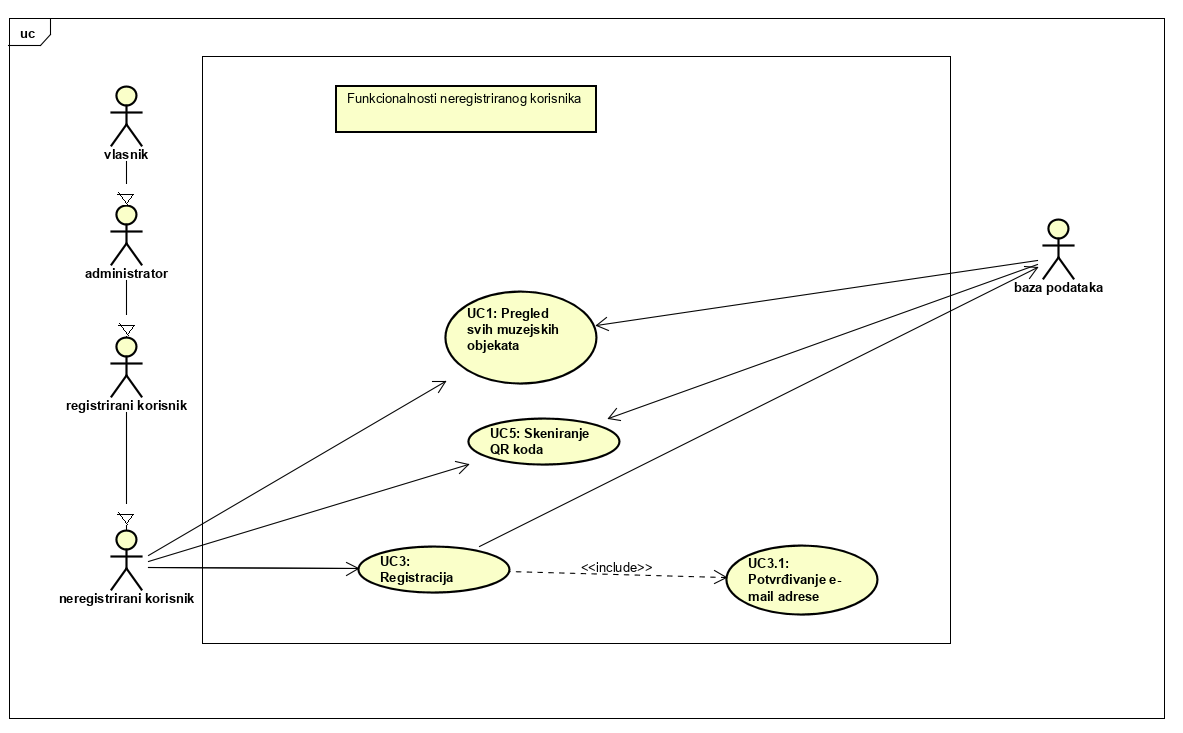
\includegraphics[scale=0.4]{slike/neregistrirani_korisnik.png}
	\centering
	\caption{Dijagram obrasca uporabe, funkcionalnosti neregistriranog korisnika}
	\label{fig:promjene}
\end{figure}

\begin{figure}[H]
	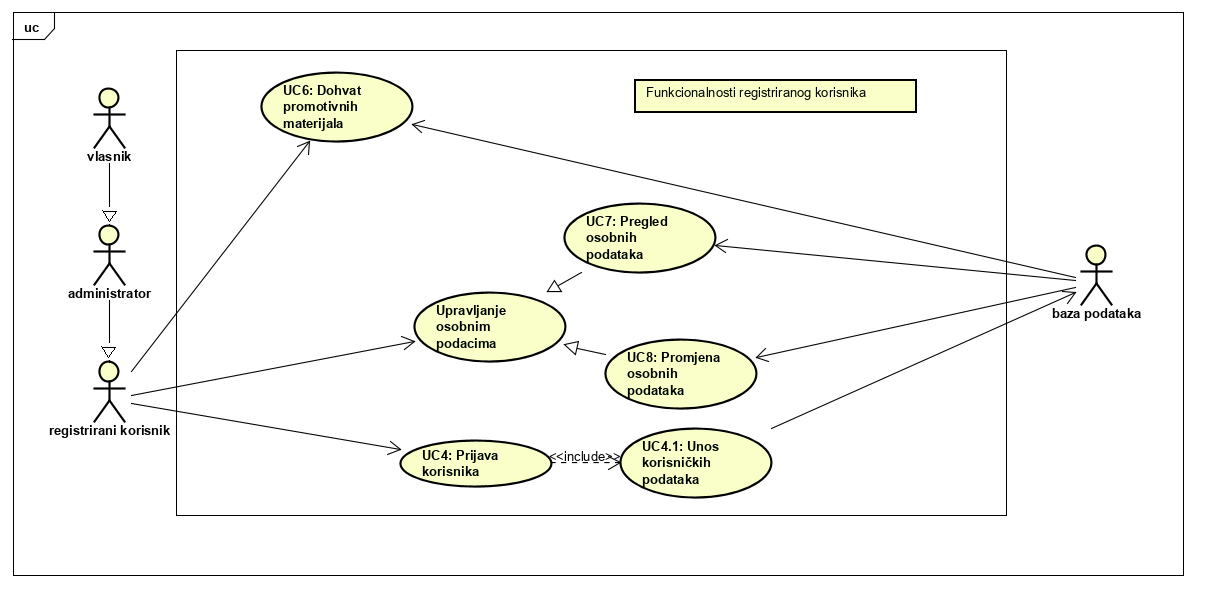
\includegraphics[scale=0.4]{slike/registrirani_korisnik.png}
	\centering
	\caption{Dijagram obrasca uporabe, funkcionalnosti registriranog korisnika}
	\label{fig:promjene}
\end{figure}	
\begin{figure}[H]
	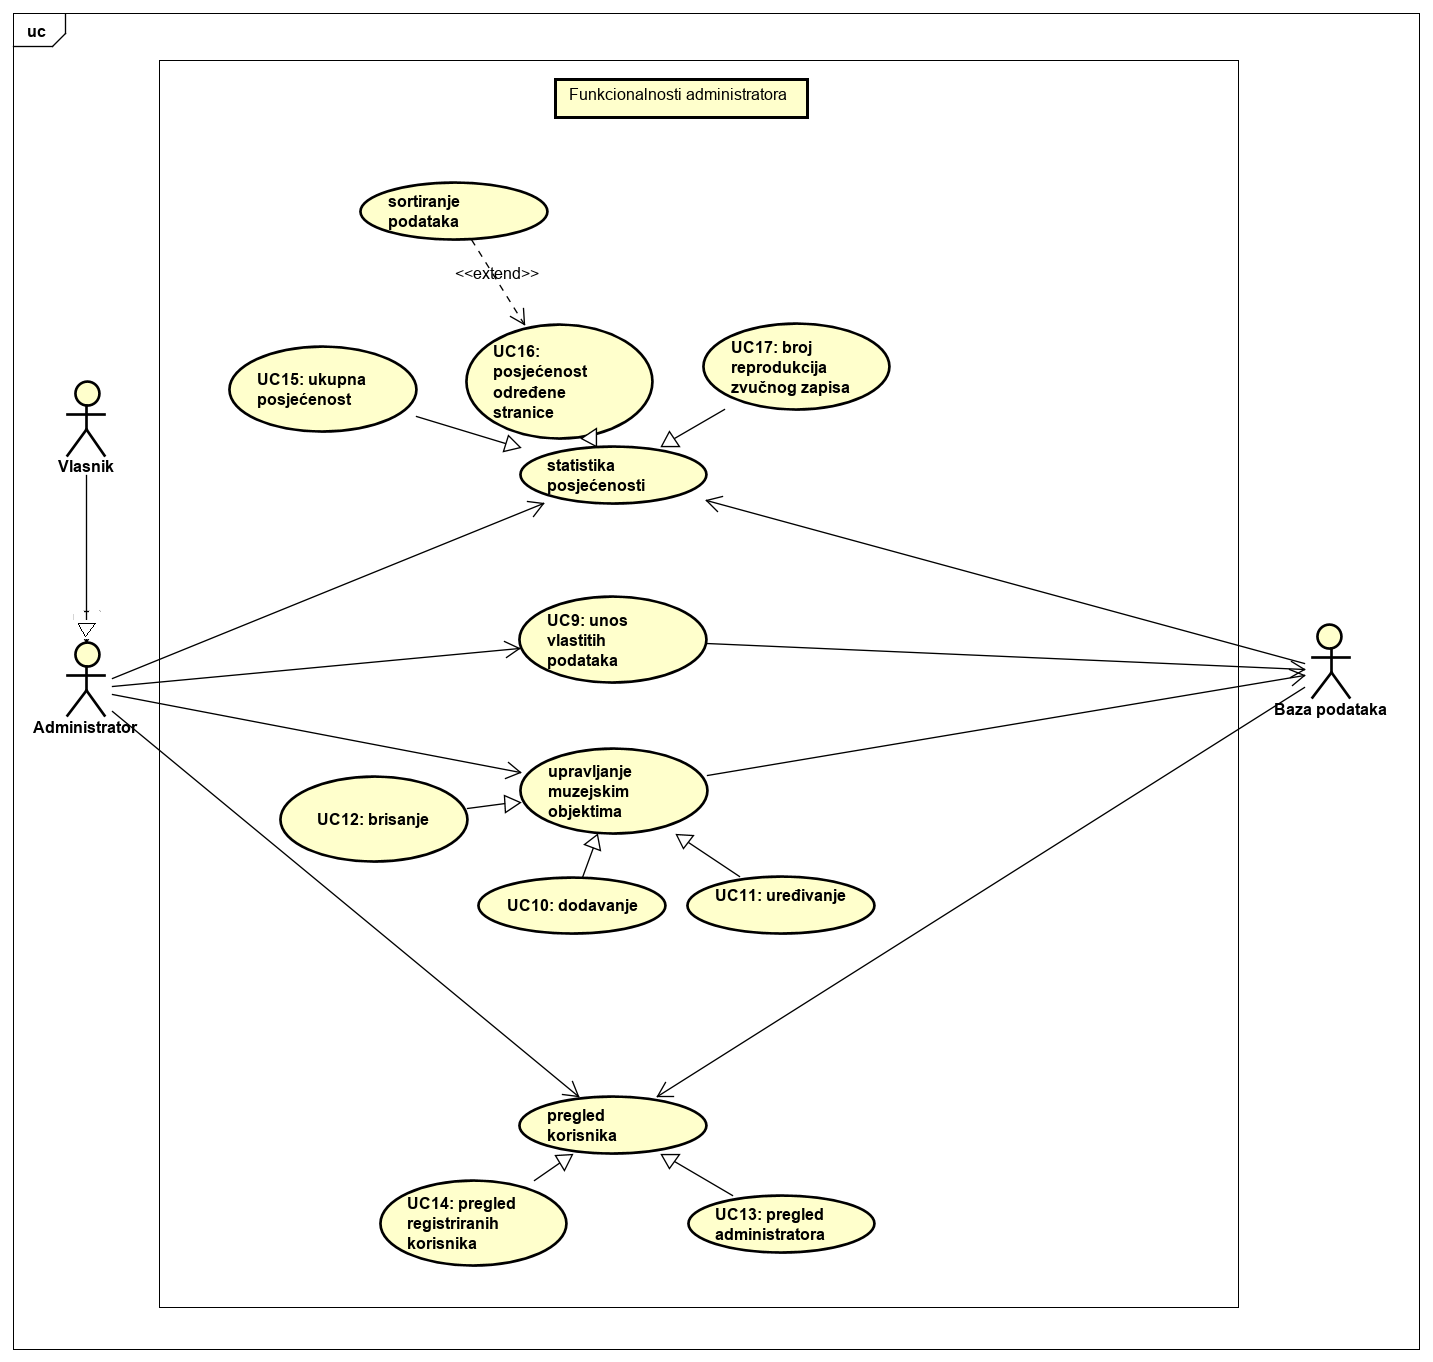
\includegraphics[scale=0.35]{slike/Administrator.png}
	\centering
	\caption{Dijagram obrasca uporabe, funkcionalnosti administratora}
	\label{fig:promjene}
\end{figure}
\begin{figure}[H]
	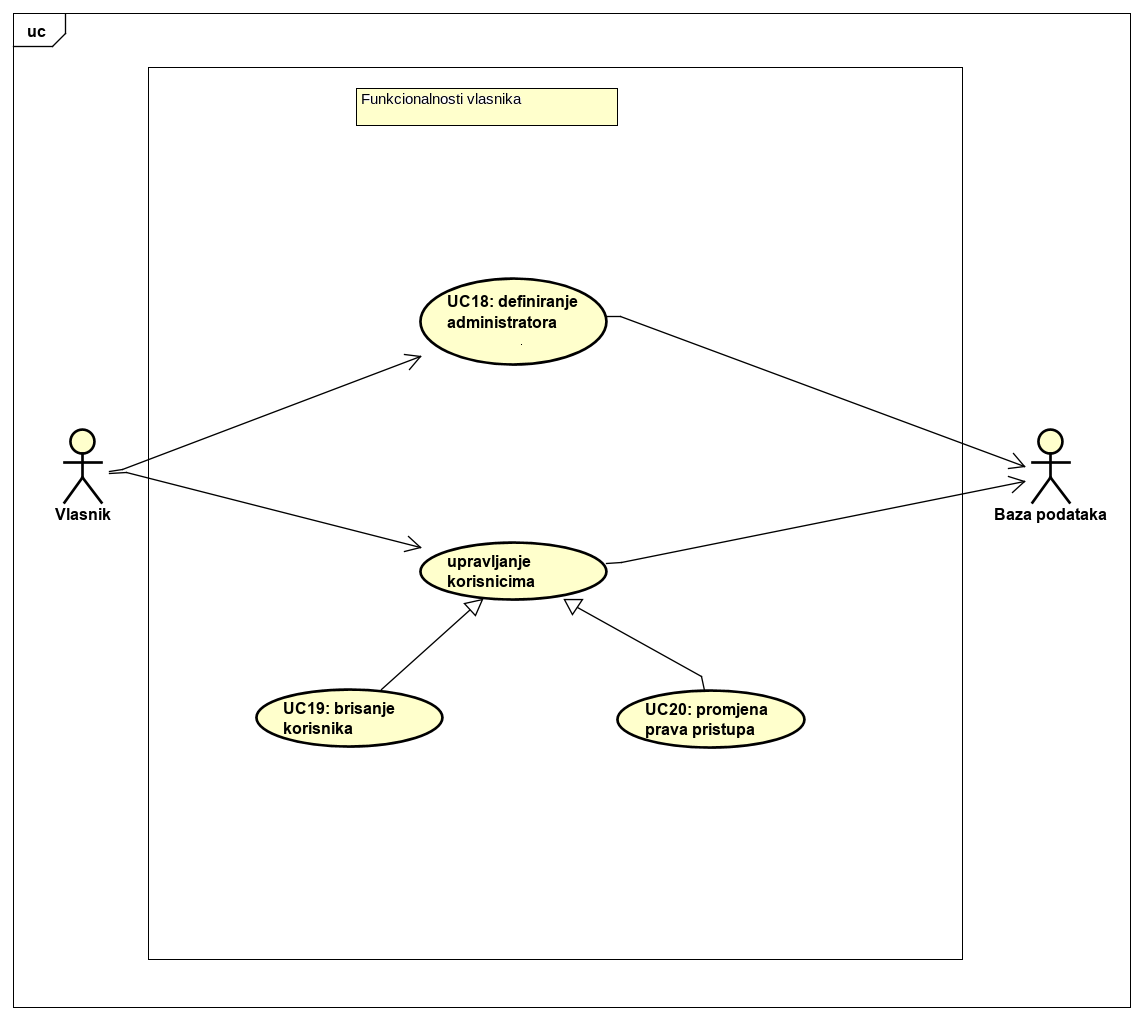
\includegraphics[scale=0.4]{slike/vlasnik.png}
	\centering
	\caption{Dijagram obrasca uporabe, funkcionalnosti vlasnika}
	\label{fig:promjene}
\end{figure}

\newpage

\subsection{Sekvencijski dijagrami}

				\begin{figure}[H]
					\textbf{Obrazac uporabe UC2 - Pregled muzejskog objekta} 
					\newline
					\newline
					Korisnik na stranici svih muzejskih objekata odabire muzejski objekt koji želi pregledati. Otvara se stranica muzejskog objekta s njegovim imenom, opisom, slikom i zvučnim zapisom. \par
					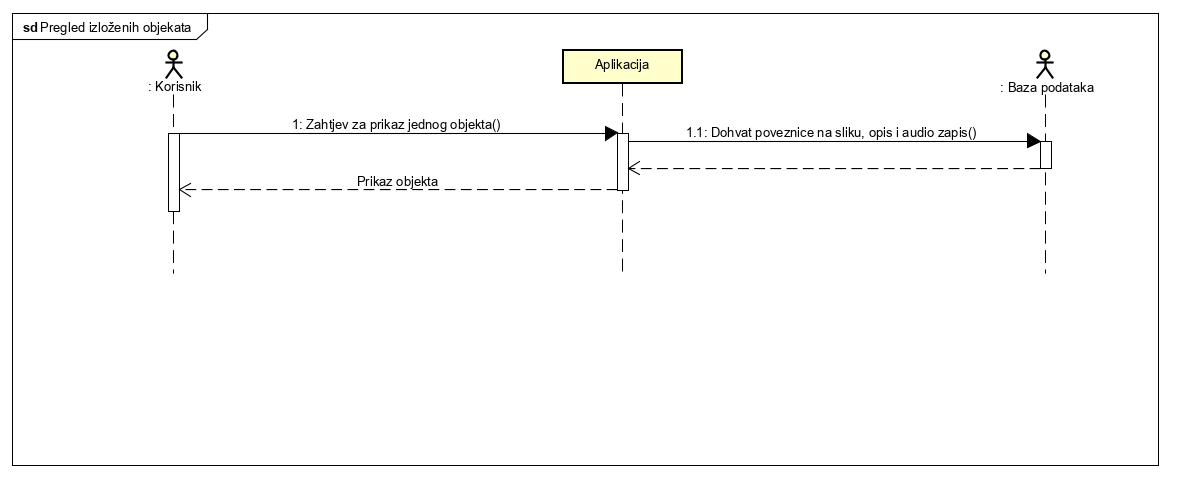
\includegraphics[width=170mm,height=100mm]{slike/Pregled_izlozenih_objekata.png} 
					\newline
					\centering
					\caption{Sekvencijski dijagram za UC2}
					\label{fig:promjene}
				\end{figure}

				\begin{figure}[H]
					\textbf{Obrazac uporabe UC3 - Registracija} 
					\newline
					\newline
					Neregistrirani korisnik odabire opciju za registraciju. Korisniku se otvara formular za registraciju. Korisnik unosi podatke u formular i potvrđuje svoj unos. Nakon korisnikove potvrde provjerava se u bazi podataka postoji li korisnik s unesenim korisničkim imenom te jesu li svi podatci ispravni. Ako korisnik već postoji ili su podatci krivo uneseni, korisniku se otvara formular za ponovni unos podataka. Ako su svi podatci ispravni korisniku se šalje mail za potvrdu podataka. Nakon potvrđivanja podataka mail adresom, podatci se unose u bazu podataka. \par
					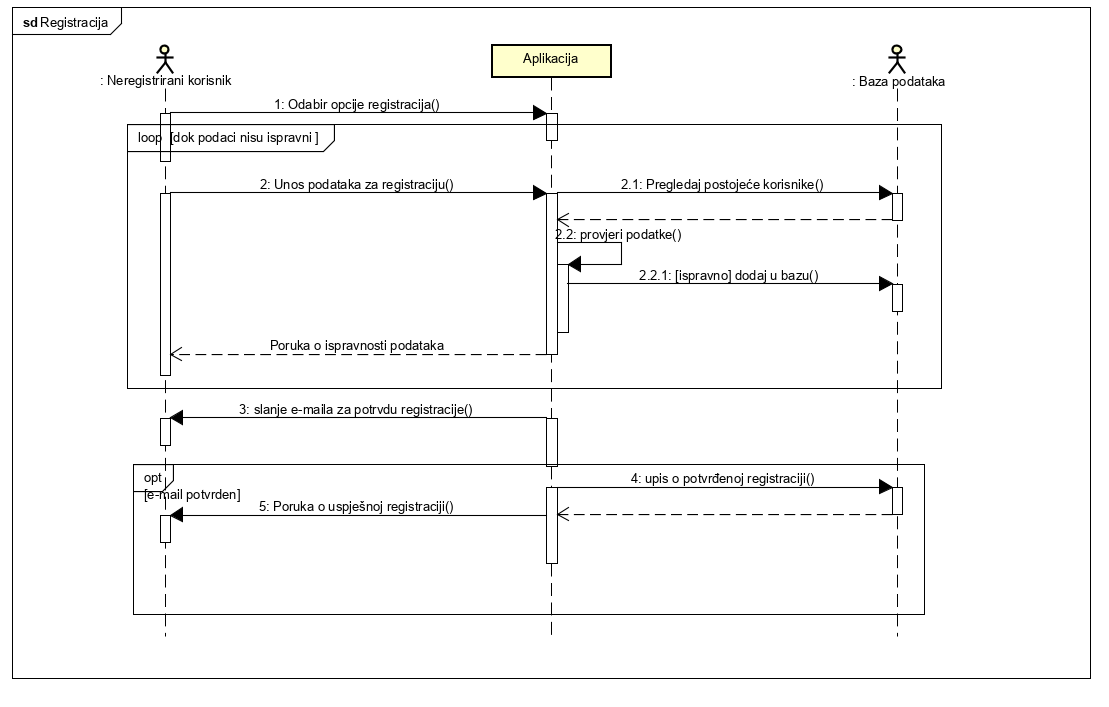
\includegraphics[width=170mm,height=100mm]{slike/Reg.png} 
					\newline
					\centering
					\caption{Sekvencijski dijagram za UC3}
					\label{fig:promjene}
				\end{figure}

                \begin{figure}[H]
                	\textbf{Obrazac uporabe UC4 - Prijava korisnika} 
                	\newline
                	\newline
                	Neprijavljeni korisnik odabire opciju za prijavu. Korisniku se otvara formular za prijavu. Korisnik unosi podatke u formular i potvrđuje svoj unos. Nakon korisnikove potvrde provjerava se u bazi podataka postoji li korisnik s unesenim korisničkim imenom te je li unesena ispravna lozinka. Ako korisnik ne postoji ili lozinka nije ispravna, korisniku se otvara formular za ponovni unos podataka. Ako su svi podatci ispravni korisniku se otvara početna stranica i prijavljen je u sustav. \par
                	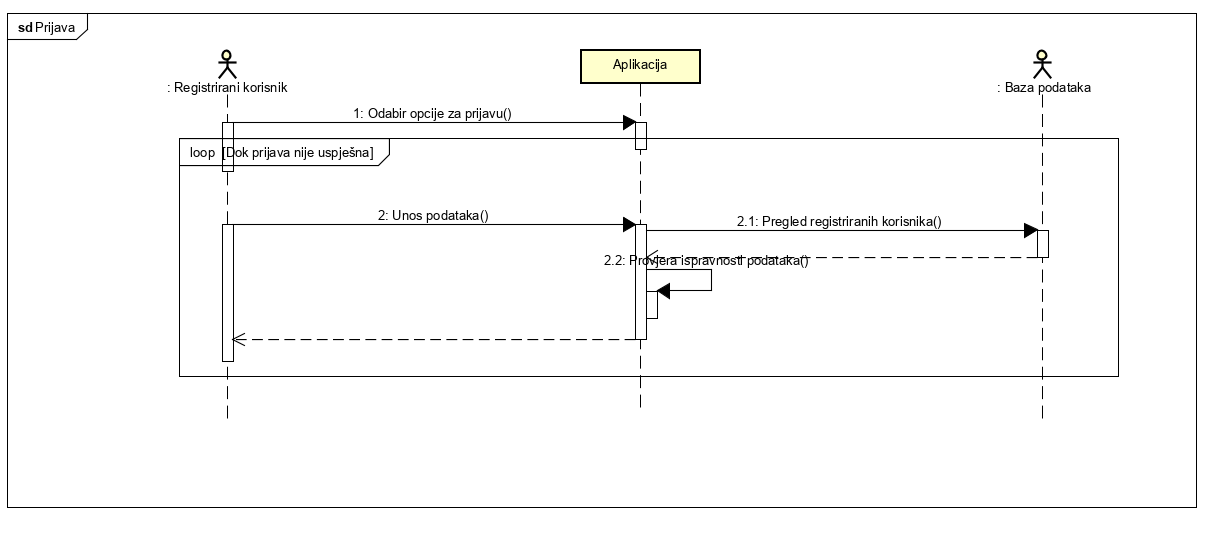
\includegraphics[width=170mm,height=100mm]{slike/Prijava.png} 
                	\newline
					\centering
					\caption{Sekvencijski dijagram za UC4}
					\label{fig:promjene}
				\end{figure}
			
			
				\begin{figure}[H]
					\textbf{Obrazac uporabe UC18 - Definiranje administratora} 
					\newline
					\newline
					Vlasnik odabire opciju za dodavanje administratora. Otvara se formular s podatcima o administratoru. Vlasnik unosi podatke o administratoru i potvrđuje unos. Provjerava se ispravnost unesenih podataka. Ako podatci nisu ispravni otvara se formular za ponovni unos podataka. Ako su podatci ispravni pohranjuju se u bazu podataka te se vlasniku otvara stranica na kojoj je popis svih administratora. \par
					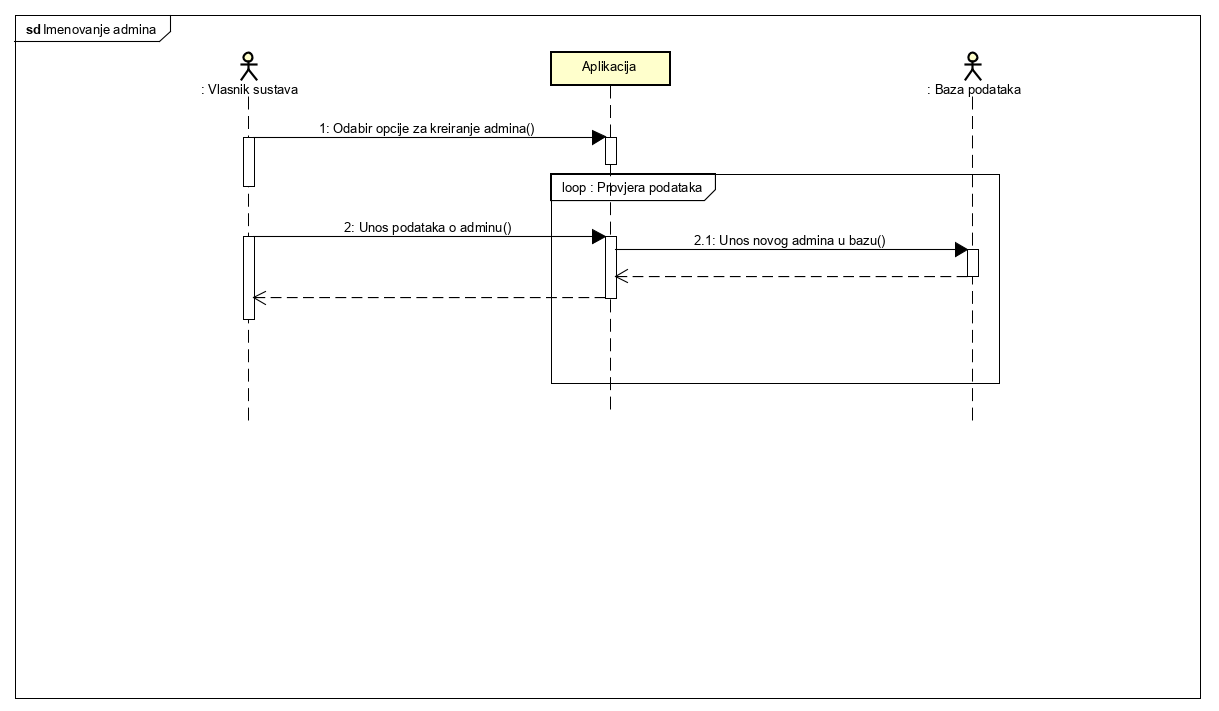
\includegraphics[width=170mm,height=100mm]{slike/Imenovanje_admina.png} 
					\newline
					\centering
					\caption{Sekvencijski dijagram za UC18}
					\label{fig:promjene}
				\end{figure}
			
				\begin{figure}[H]
					\textbf{Obrazac uporabe UC9 - Unos vlastitih podataka} 
					\newline
					\newline
					Administrator se prijavljuje u sustav te odabire opciju izmjena vlastitih podataka. Otvara se formular s osobnim podatcima. Administrator unosi podatke u formular i potvrđuje svoj unos. Nakon potvrde provjerava se jesu li svi podatci ispravni. Ako podatci nisu ispravni, korisniku se otvara formular za ponovni unos podataka. Ako su svi podatci ispravni podatci se unose u bazu podataka te se administratoru otvara početna stranica. \par
					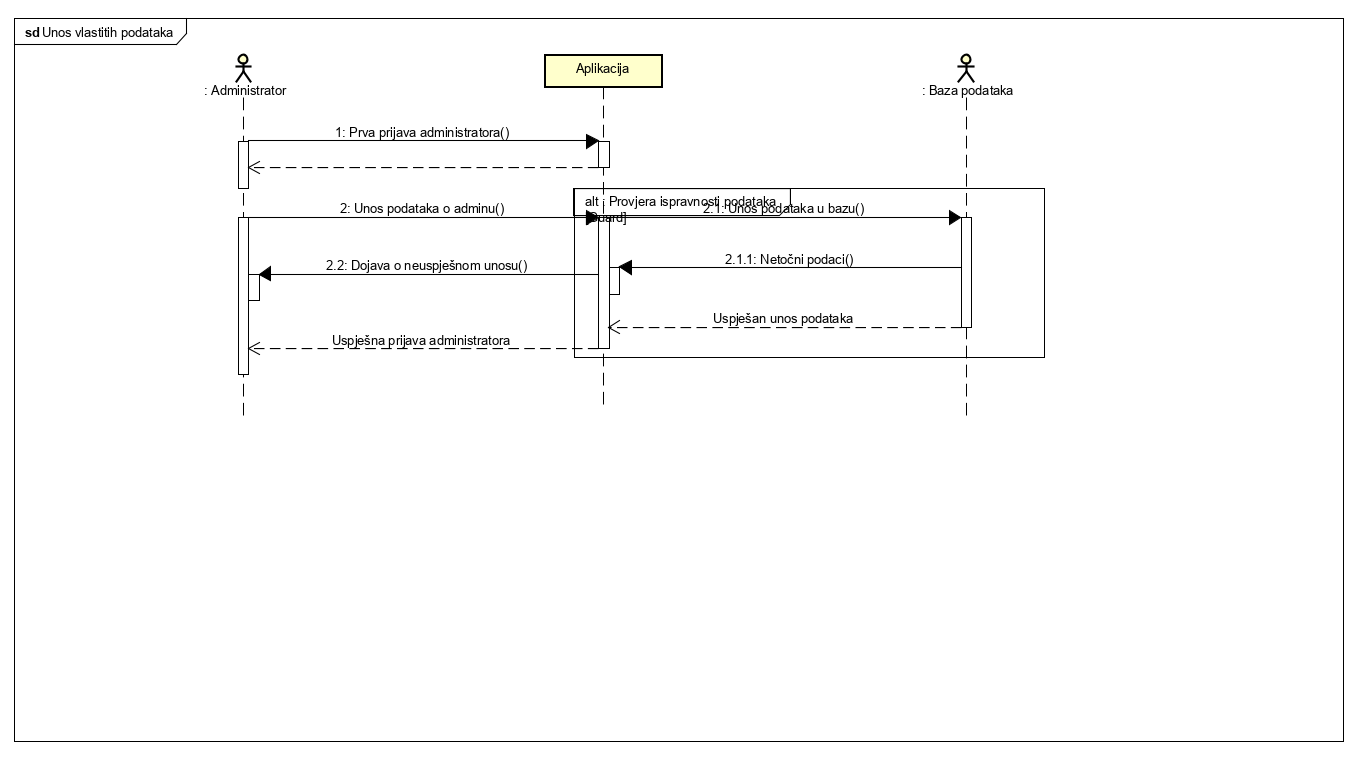
\includegraphics[width=170mm,height=100mm]{slike/Unos_vlastitih_podataka.png} 
					\newline
					\centering
					\caption{Sekvencijski dijagram za UC9}
					\label{fig:promjene}
				\end{figure}
				
				\begin{figure}[H]
					\textbf{Obrazac uporabe UC12 - Brisanje muzejskog objekta} 
					\newline
					\newline
					Administrator odabire jedan muzejski objekt te aplikacija dohvaća podatke o tom objektu iz baze podataka i prikazuje ih na zaslonu. Administrator odabire opciju brisanja tog objekta. Baza podataka briše sve podatke vezane za taj objekt (slika, opis, audio zapis). Aplikacija na zaslon ispisuje poruku o uspješnom brisanju objekta. \par
					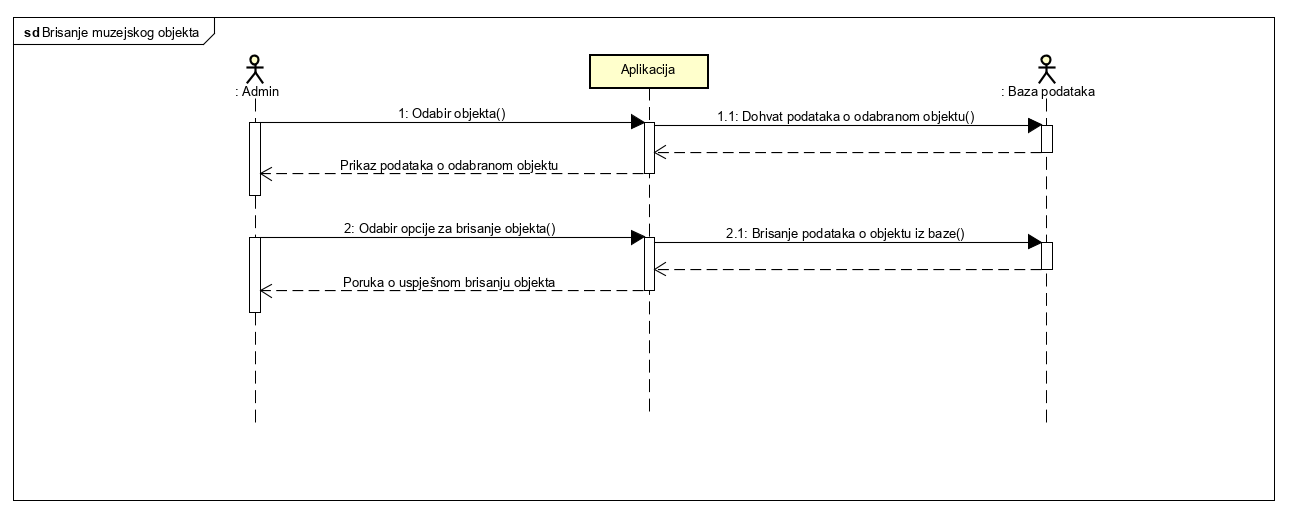
\includegraphics[width=170mm,height=100mm]{slike/Brisanje_muzejskog_objekta.png} 
					\newline
					\centering
					\caption{Sekvencijski dijagram za UC12}
					\label{fig:promjene}
				\end{figure}
				
				\begin{figure}[H]
					\textbf{Obrazac uporabe UC11 - Uređivanje podataka o muzejskom objektu} 
					\newline
					\newline
				    Administrator odabire jedan muzejski objekt koji želi urediti te mu aplikacija prikazuje podatke o tom objektu koje dohvaća iz baze podataka. Administrator unosi nove podatke te aplikacija vrši provjeru unesenih podataka. Ako su podaci ispravni, oni se unose u bazu podataka i administrator od aplikacije dobiva poruku o uspješnom unosu. Ako su podaci neispravni, administratoru se na zaslonu prikazuje poruka o neuspješnoj promjeni zbog neispravnih podataka. \par
					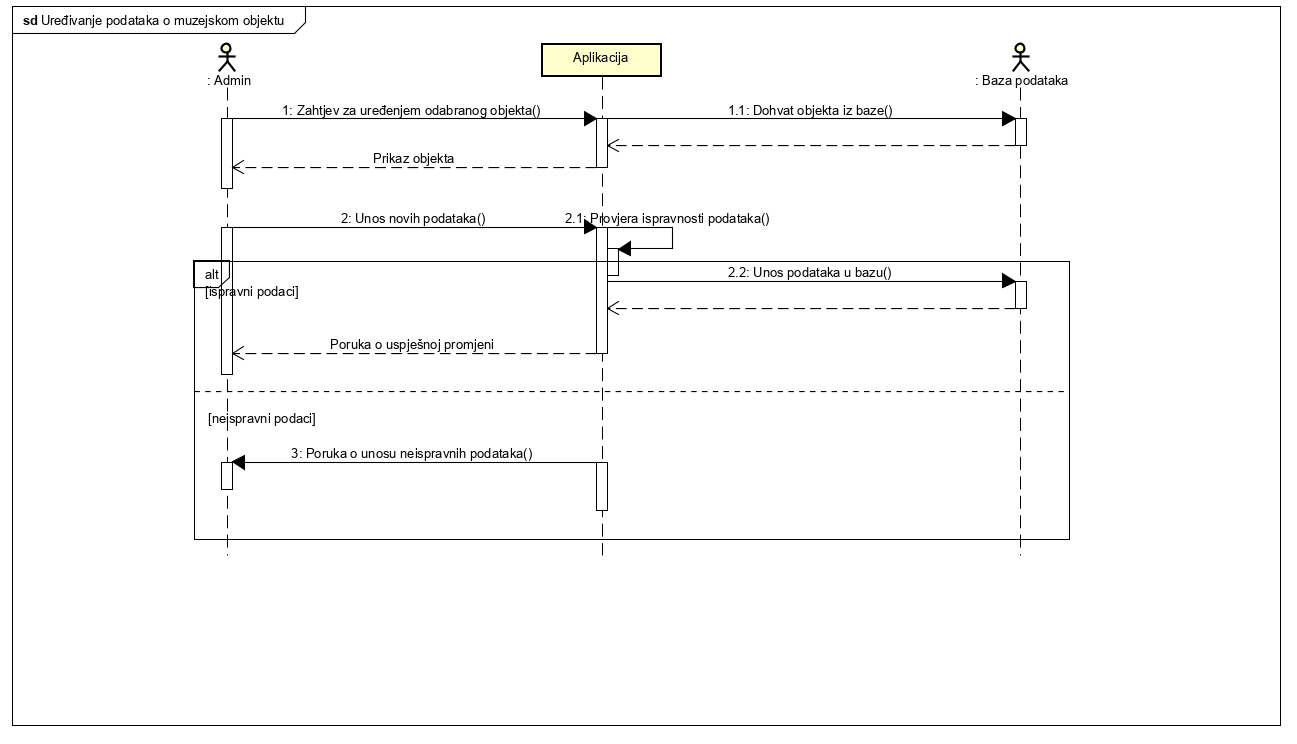
\includegraphics[width=170mm,height=100mm]{slike/Uredivanje_podataka_o_muzejskom_objektu.png} 
					\newline
					\centering
					\caption{Sekvencijski dijagram za UC11}
					\label{fig:promjene}
				\end{figure}



\newpage
\section{Ostali zahtjevi}

	\begin{packed_item}

		\item {U sustavu je omogućen paralelni rad vlasnika, administratora \newline te svih korisnika}
		\item {Neispravnost korištenja sustava ne smije utjecati na sustav ili bazu podataka}
		\item {Autorizacija za određene korisnike (akcije koje su im odobrene)}
		\item {Korištenje hrvatskog jezika i podrživost svih znakova hrvatske abecede}
		\item {Korisnik ne smije biti u bazi registranih korisnika ukoliko nije \newline potvrdio e-mail adresu}
		\item {Neograničen broj registriranih korisnika}
		\item {Najveća duljina audiozapisa je 3 minute}
		\item {Poboljšanja dodavana u novijim verzijama ne smiju narušiti trenutne \newline zadaće sustava}
		\item {Pregled podataka i slušanje audiozapisa omogućen svim \newline posjetiteljima stranice}
		\item {Dostupnost promo materijalima samo registriranim korisnicima}
		\item {Vlasnik i administratori vide broj trenutno aktivnih administratora i \newline aktivnih registriranih korisnika}
		\item {Administratori i vlasnik vide koliko puta je određeni audiozapis reproduciran}
	
	\end{packed_item}



